\section{Selective Symbolic Execution}\label{sec:s2e}

% -------- symbolic execution -------- %
\textbf{Symbolic execution} is an advanced analysis technique particularly suited for automated software testing \todo{ct} and malware analysis \todo{ct}.
Instead of concrete input (7, ``string'', ...) symbolic execution uses symbolic values ($\lambda$, $\beta$, ...) when processing code.
Assignments in the program path have impacts on these symbolic values.
The integer calculation $x = x - 2$, for instance, would update the symbolic expression representing the input $x$ to $\lambda - 2$.
Conditional statements (if <condition> then ... else ...) fork program execution into two new paths.
Both paths are then constrained by an additional condition, the `then' branch with the if-condition and the `else' branch with the negated if-condition respectively.
\todo{Bild > Text}

\begin{figure}
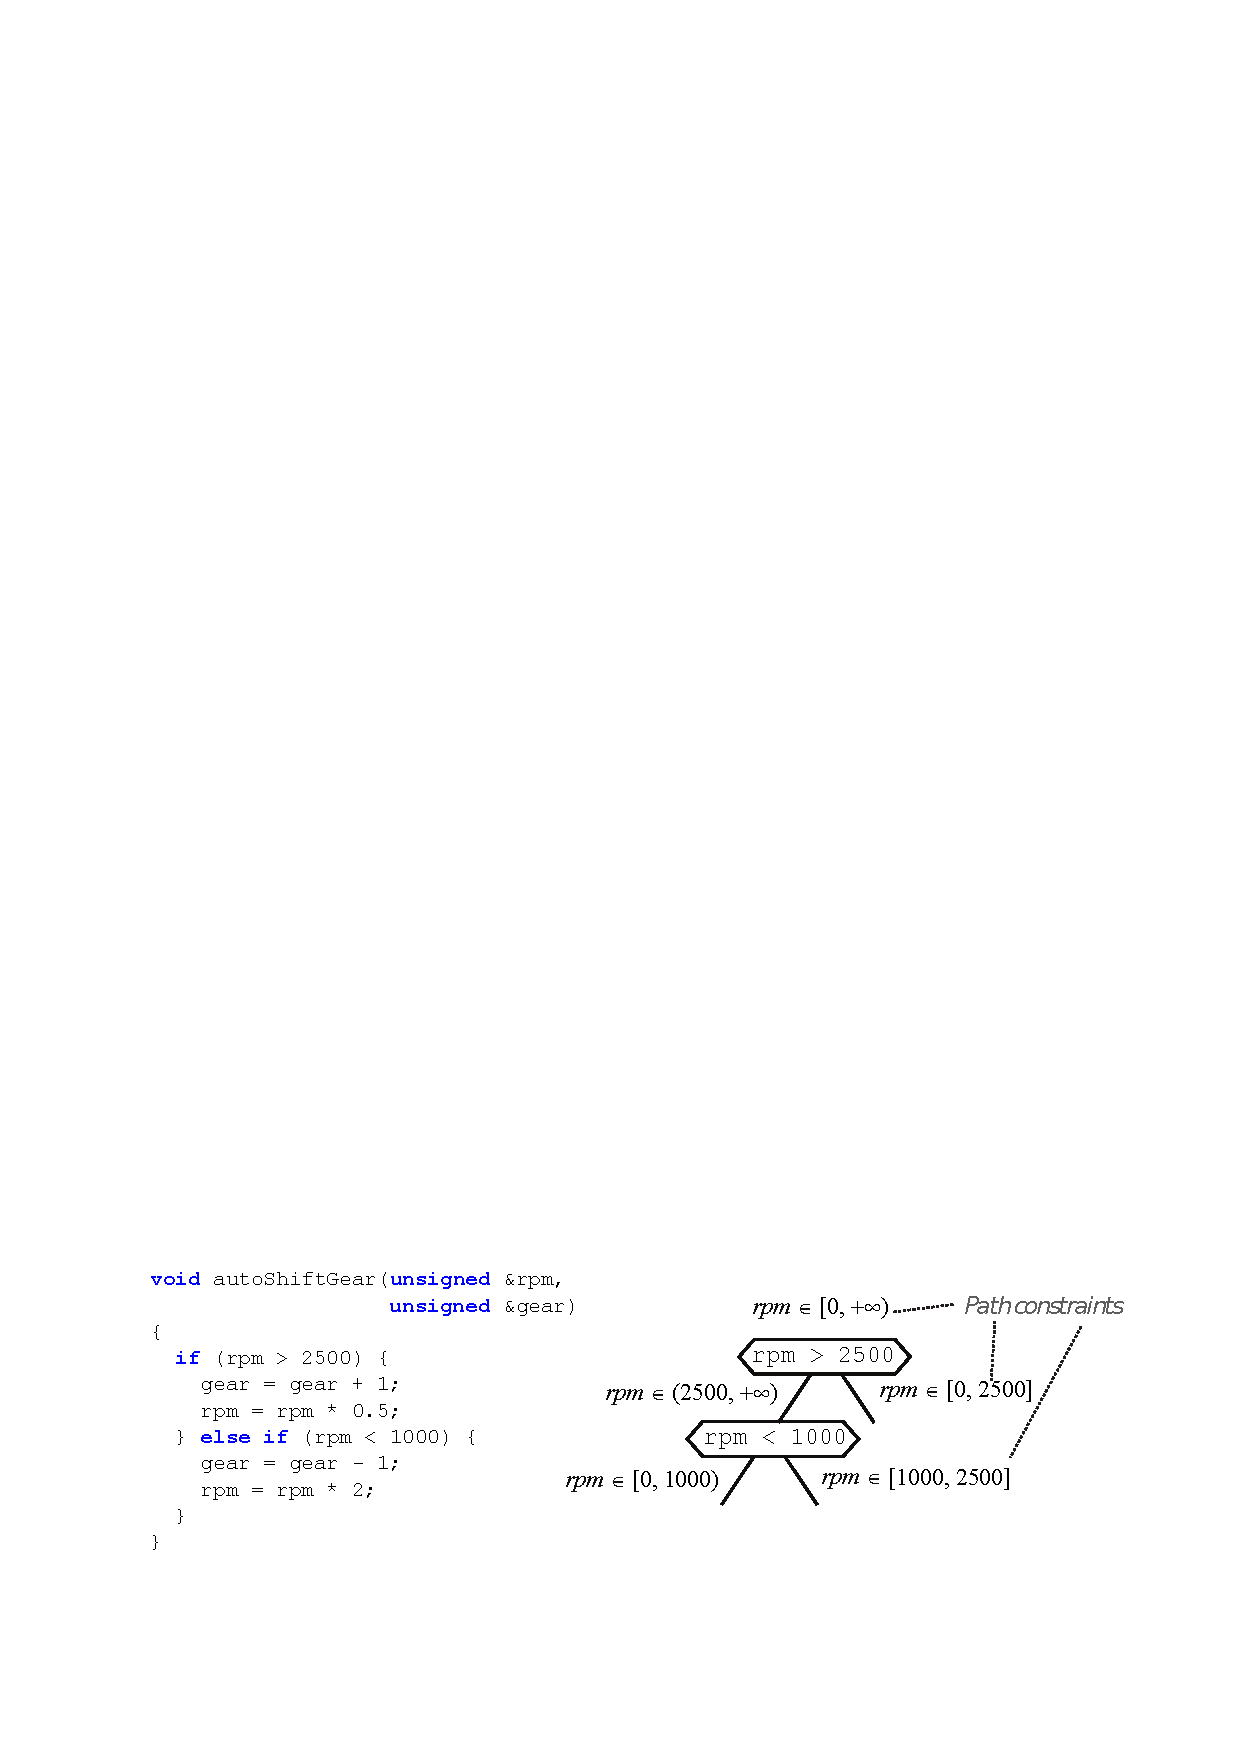
\includegraphics[width=\columnwidth]{symb_exe_2}
\caption{Execution tree with path constraints for the symbolic variable $rpm$ \cite{chip14s2e}}
\label{fig:arch}
\end{figure}

Following this procedure results in a tree-like structure of constrained symbolic expressions.
A constraint solver can now take all constraints along one execution path as input and find one concrete input (e.g., $\lambda = 5$) which would lead to the program following exactly this path.
Such results greatly alleviate writing reproducible test cases \cite{chip09sel}.

On a technical level, symbolic execution engines save state information (program memory, constraint information, ...) in a custom data structure.
Each conditional statement involving symbolic values results in a $fork$ of the program state.
The two newly created branches are completely independent and can therefore be processed in parallel.

% -------path explosion
But the exponential growth of conditionals soon reveals scaling problems of this forking strategy.
Despite heavy research on optimisations mitigating this \textit{path explosion} problem \todo{ct} only relatively small programs ($\cong$ thousands of lines of code) can be analysed symbolically \cite{chip09sel}.

% -------interaction with env
%In addition to the path explosion problem, classical symbolic execution ... interaction with the environment...
Additionally, symbolic execution faces problems when the program under analysis \textit{interacts with its environment}.
If it calls a system library like $libc$, in theory the whole system stack including invoked libraries, operating system and drivers would have to be executed symbolically.
Considering the path explosion problem mentioned before, the resulting complexity makes such a profound analysis hardly feasible.

% --------standard sol
One way to solve this problem is to build abstract models of the program's environment \todo{ct}.
However, due to the complexity of real-world systems, building a model of the entire system is both tedious and unnecessary - the user usually wants to analyse one single program and not the whole system \cite{chip09sel}.

\bigskip

% -------- selective symbolic execution -------- %
In order to overcome typical problems of conventional symbolic execution, Chipounov et al.~from the Swiss Federal Institute of Technology in Lausanne (EPFL) developed the concept of \textbf{selective symbolic execution} (\sse) \cite{chip09sel}.
Based on a virtual execution platform \sse gives users the illusion of running the entire system symbolically.
By limiting the scope of interest (i.e.~which parts of the system should be executed symbolically), users can effectively restrain the path explosion problem.
Program code within this defined scope is executed symbolically, whereas out-of-scope parts, which are irrelevant to the analysis, switch to concrete execution.
%One of the main contributions of the EPFL team around Chipounov is the transparent and consistent management of switching between symbolic and concrete execution modes.

% puning for scalability -> bringen?

Definition of the scope of interest (what to execute symbolically) is highly flexible.
Users may specify whole executables, code regions, or even single variables to be executed symbolically. Everything else will be treated concretely.

%This forth and back conversion -> challenge!
But since on a technical level symbolical and concrete execution are handled very differently - concrete code may run natively while symbolic instructions need to be emulated - switching back and forth these two modes is a major challenge.
Hence one of the main contributions of the EPFL team around Chipounov is the transparent and consistent management of switching between symbolic and concrete execution modes.

\todo{kill}
\cite{chip09sel}
\cite{chip11s2e}
\cite{chip12s2e}
\cite{chip14s2e}





% -------- Konsistenzmodelle -------- %

bla bla bla



%%%%%%%%%%%%%%%%%%%%%%%%%%%%%%%%%%%%%%%%%%%%%%%%%%%%%%%
\iffalse
§2	Selective Symbolic Execution
		> Theorie-Teil
		> Was ist Symbolic Execution?
		> Was kann Selective Symbolic Execution besser?
			(Concrete -> symbolic transition usw.)
		> Konsistenzmodelle (wird hier evtl. schwierig, das richtige Maß 
			zu finden, um die Sache auf wenig Platz zu verstehen)
\fi
